%----------------------------------------------------------------------------------------
%
% A LaTeX-template for 1DV510. Modified and translated by Björn Lindenberg at LNU.
% Based on an original master thesis template created by Marcus Wilhelmsson at LNU.
%
%----------------------------------------------------------------------------------------

% Settings and document configuration

\documentclass[a4paper,12pt]{article} 
\usepackage[T1]{fontenc} 
\usepackage{times} 
\usepackage[swedish,english]{babel} 
\usepackage[utf8]{inputenc} 
\usepackage{dtk-logos} 
\usepackage{wallpaper} 
\usepackage[absolute]{textpos} 
\usepackage[top=2cm, bottom=2.5cm, left=3cm, right=3cm]{geometry} 
\usepackage[parfill]{parskip} 
\usepackage{csquotes} 
\usepackage{float} 
\usepackage{lipsum} % Used for dummy text. Can be removed.
\usepackage{listings, color}
\definecolor{mGreen}{rgb}{0,0.6,0}
\definecolor{mGray}{rgb}{0.5,0.5,0.5}
\definecolor{mPurple}{rgb}{0.58,0,0.82}
\definecolor{backgroundColour}{rgb}{0.95,0.95,0.92}

\lstdefinestyle{CStyle}{
    backgroundcolor=\color{backgroundColour},   
    commentstyle=\color{mGreen},
    keywordstyle=\color{magenta},
    numberstyle=\tiny\color{mGray},
    stringstyle=\color{mPurple},
    basicstyle=\footnotesize,
    breakatwhitespace=false,         
    breaklines=true,                 
    captionpos=b,                    
    keepspaces=true,                 
    numbers=left,                    
    numbersep=5pt,                  
    showspaces=false,                
    showstringspaces=false,
    showtabs=false,                  
    tabsize=2,
    language=C
}

% Fontsizes for section headings.
\usepackage{sectsty} 
\sectionfont{\fontsize{14}{15}\selectfont}
\subsectionfont{\fontsize{12}{15}\selectfont}
\subsubsectionfont{\fontsize{12}{15}\selectfont}

%----------------------------------------------------------------------------------------
%	This part is used for the text box on the title page
%----------------------------------------------------------------------------------------
\newsavebox{\mybox}
\newlength{\mydepth}
\newlength{\myheight}

\newenvironment{sidebar}%
{\begin{lrbox}{\mybox}\begin{minipage}{\textwidth}}%
{\end{minipage}\end{lrbox}%
 \settodepth{\mydepth}{\usebox{\mybox}}%
 \settoheight{\myheight}{\usebox{\mybox}}%
 \addtolength{\myheight}{\mydepth}%
 \noindent\makebox[0pt]{\hspace{-20pt}\rule[-\mydepth]{1pt}{\myheight}}%
 \usebox{\mybox}}

%----------------------------------------------------------------------------------------
%	Title
%----------------------------------------------------------------------------------------
\newcommand\BackgroundPic{
    \put(-2,-3){
    
\includegraphics[keepaspectratio,scale=0.3]{img/lnu_etch.png} % Background image
    }
}
\newcommand\BackgroundPicLogo{
    \put(30,740){
    
\includegraphics[keepaspectratio,scale=0.10]{img/logo.png} % LNU logo
    }
}

\title{
\vspace{-8cm}
\begin{sidebar}
    \vspace{10cm}
    \normalfont \normalsize
    \huge Computer Technology I\\ % Main title
    \vspace{-1.3cm}
\end{sidebar}
\vspace{3cm}
\begin{flushleft}
    \huge Lab. 6 : CyberTech Wall Display % Subtitle
     \small \\ \emph{}
\end{flushleft}
\null
\vfill
\begin{textblock}{5}(10,13)
\begin{flushright}
\begin{minipage}{\textwidth}
\begin{flushleft} \large
\emph{Author:}\textsc{Anas Kwefati}\\  % Author
\emph{Supervisor:}  \textsc{Anders Haggren} \\  % Author
\emph{Semester:} Autumn 2019\\ % Semester
\emph{Area:} Computer Science \\ % Area
\emph{Course code:} 1DT301 % Course
\end{flushleft}
\end{minipage}
\end{flushright}
\end{textblock}
}

\date{} % Empty date command. Use \today inside for today's date.
\author{} % Normally one would use this to define authors. However in this case the title command takes care of everything, so we leave the field empty to get rid of warnings. 

\begin{document}

\pagenumbering{gobble} % Turn off page numbering
\newgeometry{left=5cm}
\AddToShipoutPicture*{\BackgroundPic} % Adds the background image to the title page
\AddToShipoutPicture*{\BackgroundPicLogo} % Adds the logo to the title page
\maketitle % Prints the title
\restoregeometry
\clearpage

\pagenumbering{roman} % Roman page numbering for abstract page


\selectlanguage{english}

\newpage

\pagenumbering{gobble} % Turn off page numbering
\tableofcontents 

\newpage
\pagenumbering{arabic} % Turn on page numbering

%TASK1
\section{Task 1}
\lstset{style=CStyle}

\begin{lstlisting}[style=CStyle]
/*>>>>>>>>>>>>>>>>>>>>>>>>>>>>>>>>>>>>>>>>>>>>>>>>>>>>>>>>>>>
; 1DT301, Computer Technology I
; Date: 2016-09-15
; Author:
;    Anas Kwefati
;
; Lab number: 6
; Title: CyberTech Wall Display
;
; Hardware: STK600, CPU ATmega2560
;
; Function: Program that writes a character on the CyberTech Display.
;
; Input ports: none
;
; Output ports: CyberTech Display.
;
; Subroutines:
; Included files: <avr/io.h>
;
;Other information: Display is connected to the serial port (RS232) on the STK600.
; Communication speed is 2400bps.
;Changes in program: (Description and date)
<<<<<<<<<<<<<<<<<<<<<<<<<<<<<<<<<<<<<<<<<<<<<<<<<<<<<<<<<<<*/

#include <avr/io.h>
#include <stdio.h>
#include <string.h>
//#include <util/delay.h>
#define FCPU 1000000// Clock Speed
#define BAUD 2400 //Communication Speed Display rate 2400
#define MYUBBRR (FCPU/16/BAUD-1) //UBBRR = 25 -> osc = 1MHz and UBRR = 47 -> osc = 1,843200MHz

void uart_int(void);
void toPutty(unsigned char data);

int main(void)
{
    uart_int();
    
    char* txt = "\rAO0001Hi How are you ? :)";
    int checksum =0;
    //We make sure that everything is in it
    for(int i =0; i<strlen(txt);i++){
        checksum += txt[i];
    }
    
    checksum\%=256;
    
    char toDisplay [strlen(txt)+3];
    sprintf(toDisplay, "\%s\%02X\n", txt, checksum); //\%02x means print at least 2 digits, prepends it with 0's if there's less.
    //\%02x is used to convert one character to a hexadecimal string
    
    for (int i = 0; i<strlen(txt)+3;i++){
        toPutty(toDisplay[i]);
    }
    
    txt = "\rZD0013C\n";
    for(int i = 0; i<strlen(txt);i++){
        toPutty(txt[i]);
    }
    
    return 0;
}

//INITALIZATION OF THE DISPLAY

void toPutty(unsigned char data){
    //WAIT FOR DATA TO BE RECEIVED
    while(!(UCSR1A & (1<<UDRE1)));
    UDR1 = data;
}

void uart_int(void) {
    UBRR1L = MYUBBRR; //25 because we are setting the board at 1MHz
    /*Enable receiver and transmitter*/
    UCSR1B = (1<<RXEN1|1<<TXEN1); // Receive Enable (RXEN) bit // Transmit Enable (TXEN) bit
}


\end{lstlisting}

\break
\begin{figure}
\begin{center}
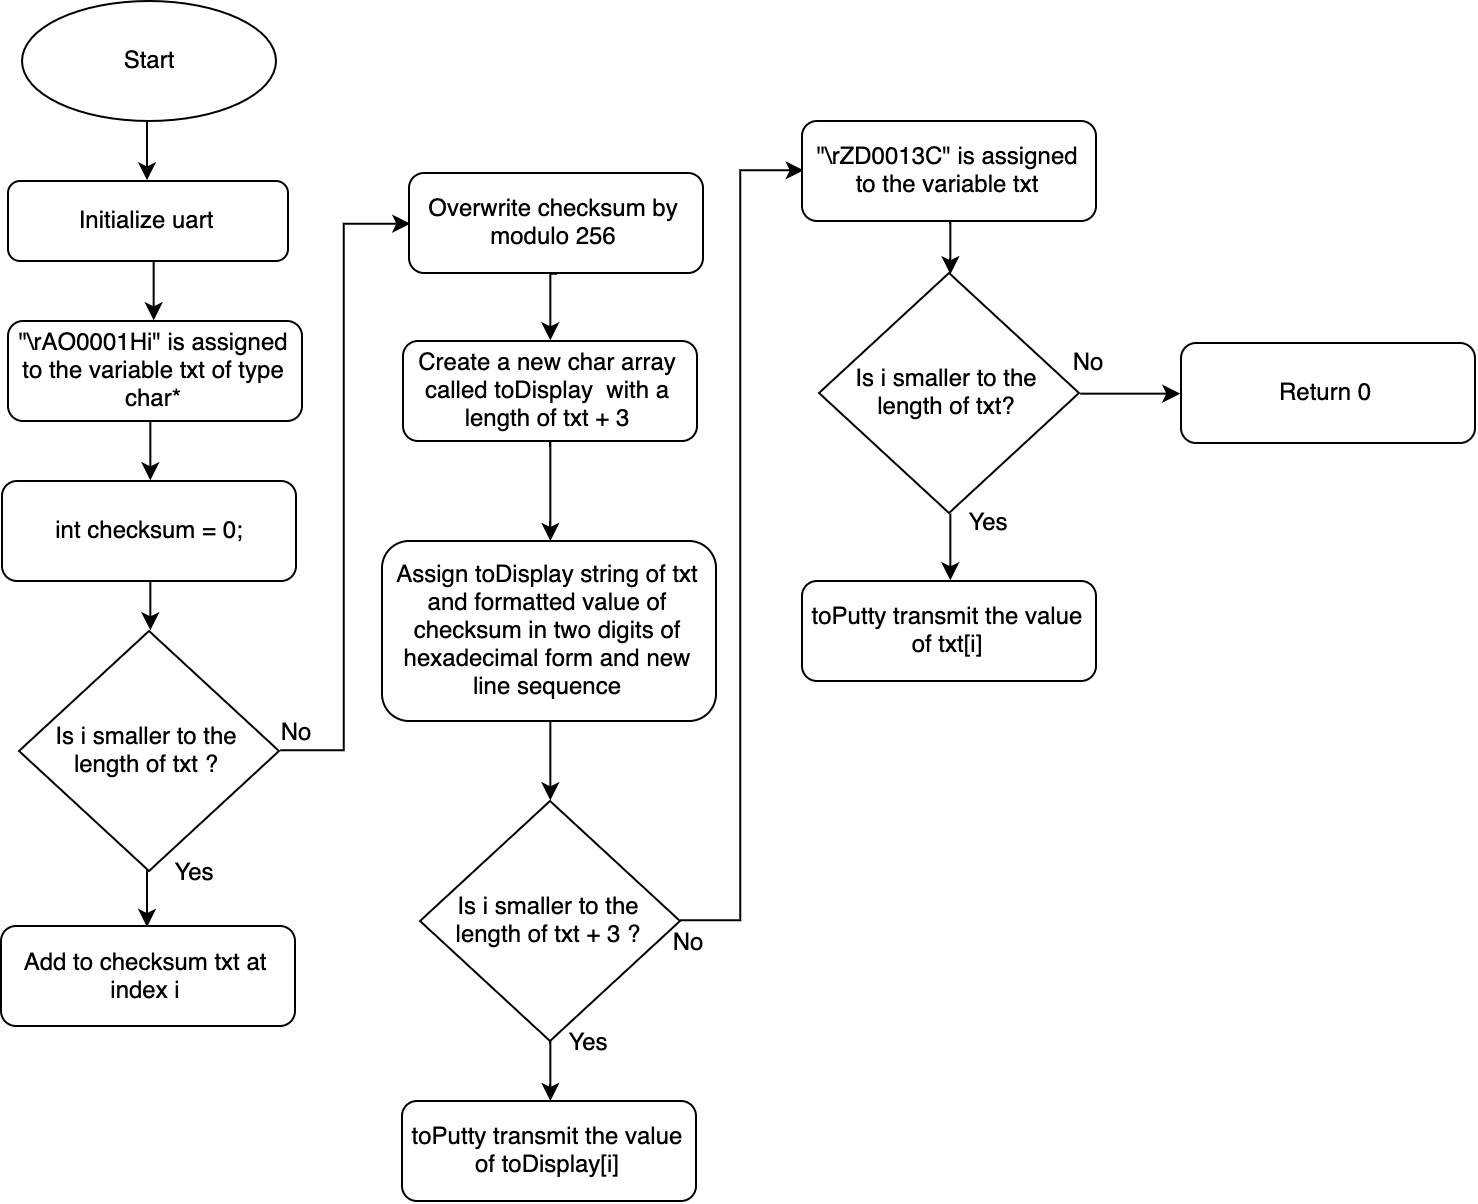
\includegraphics[width=\textwidth/1 ]{flowchart/task1_flowchart.png}
\end{center}
\caption{Task 1 flowchart}
\label{task1}
\end{figure}



%TASK2
\section{Task 2}
In this task we used the same methods for uart\_int(void) and toPutty(unsigned char data). 
\lstset{style=CStyle}

\begin{lstlisting}[style=CStyle]
/*>>>>>>>>>>>>>>>>>>>>>>>>>>>>>>>>>>>>>>>>>>>>>>>>>>>>>>>>>>>
; 1DT301, Computer Technology I
; Date: 2016-09-15
; Author:
;    Anas Kwefati
;
; Lab number: 6
; Title: CyberTech Wall Display
;
; Hardware: STK600, CPU ATmega2560
;
; Function: Program that writes characters on all text lines on the CyberTech Display.
; The program will write to all 3 rows.
;
; Input ports: none
;
; Output ports: CyberTech Display.
;
; Subroutines:
; Included files: <avr/io.h>
;
;Other information: Display is connected to the serial port (RS232) on the STK600.
; Communication speed is 2400bps.
;Changes in program: (Description and date)
<<<<<<<<<<<<<<<<<<<<<<<<<<<<<<<<<<<<<<<<<<<<<<<<<<<<<<<<<<<*/

#include <avr/io.h>
#include <stdio.h>
#include <string.h>
//#include <util/delay.h>
#define FCPU 1000000// Clock Speed
#define BAUD 2400 //Communication Speed Display rate 2400
#define MYUBBRR (FCPU/16/BAUD-1) //UBBRR = 25 -> osc = 1MHz and UBRR = 47 -> osc = 1,843200MHz

void uart_int(void);
void toPutty(unsigned char data);
void toDisplayOnLCD(char* stringChar);

int main(void)
{
	uart_int();
	
	char* txt = "\rAO0001First Line              Second Line";
	
	toDisplayOnLCD(txt);
	

	
	txt = "\rBO0001Third Line";
	toDisplayOnLCD(txt);
	
	txt = "\rZD0013C\n";
	toDisplayOnLCD(txt);
	
	return 0; 
}


//METHOD TO DISPLAY ON THE SCREEN 
void toDisplayOnLCD(char* stringChar){
	
	int checksum = 0; 
	 //We make sure that everything is in it
	 for(int i =0; i<strlen(stringChar);i++){
		 checksum += stringChar[i];
	 }
	 
	 checksum\%=256;
	 
	 char toDisplay [strlen(stringChar)+3];
	 sprintf(toDisplay, "\%s\%02X\n", stringChar, checksum); //\%02x means print at least 2 digits, prepends it with 0's if there's less.
	 //\%02x is used to convert one character to a hexadecimal string
	
	for (int i = 0; i<strlen(stringChar)+3;i++){
		toPutty(toDisplay[i]);
	}
}

//INITIALIZATION OF THE DISPLAY 

void toPutty(unsigned char data){
	//WAIT FOR DATA TO BE RECEIVED
	while(!(UCSR1A & (1<<UDRE1)));
	UDR1 = data;
}

void uart_int(void) { 
	UBRR1L = MYUBBRR; //25 because we are setting the board at 1MHz
	/*Enable receiver and transmitter*/
	UCSR1B = (1<<RXEN1|1<<TXEN1); // Receive Enable (RXEN) bit // Transmit Enable (TXEN) bit
}




\end{lstlisting}
\break
\begin{figure}
\begin{center}
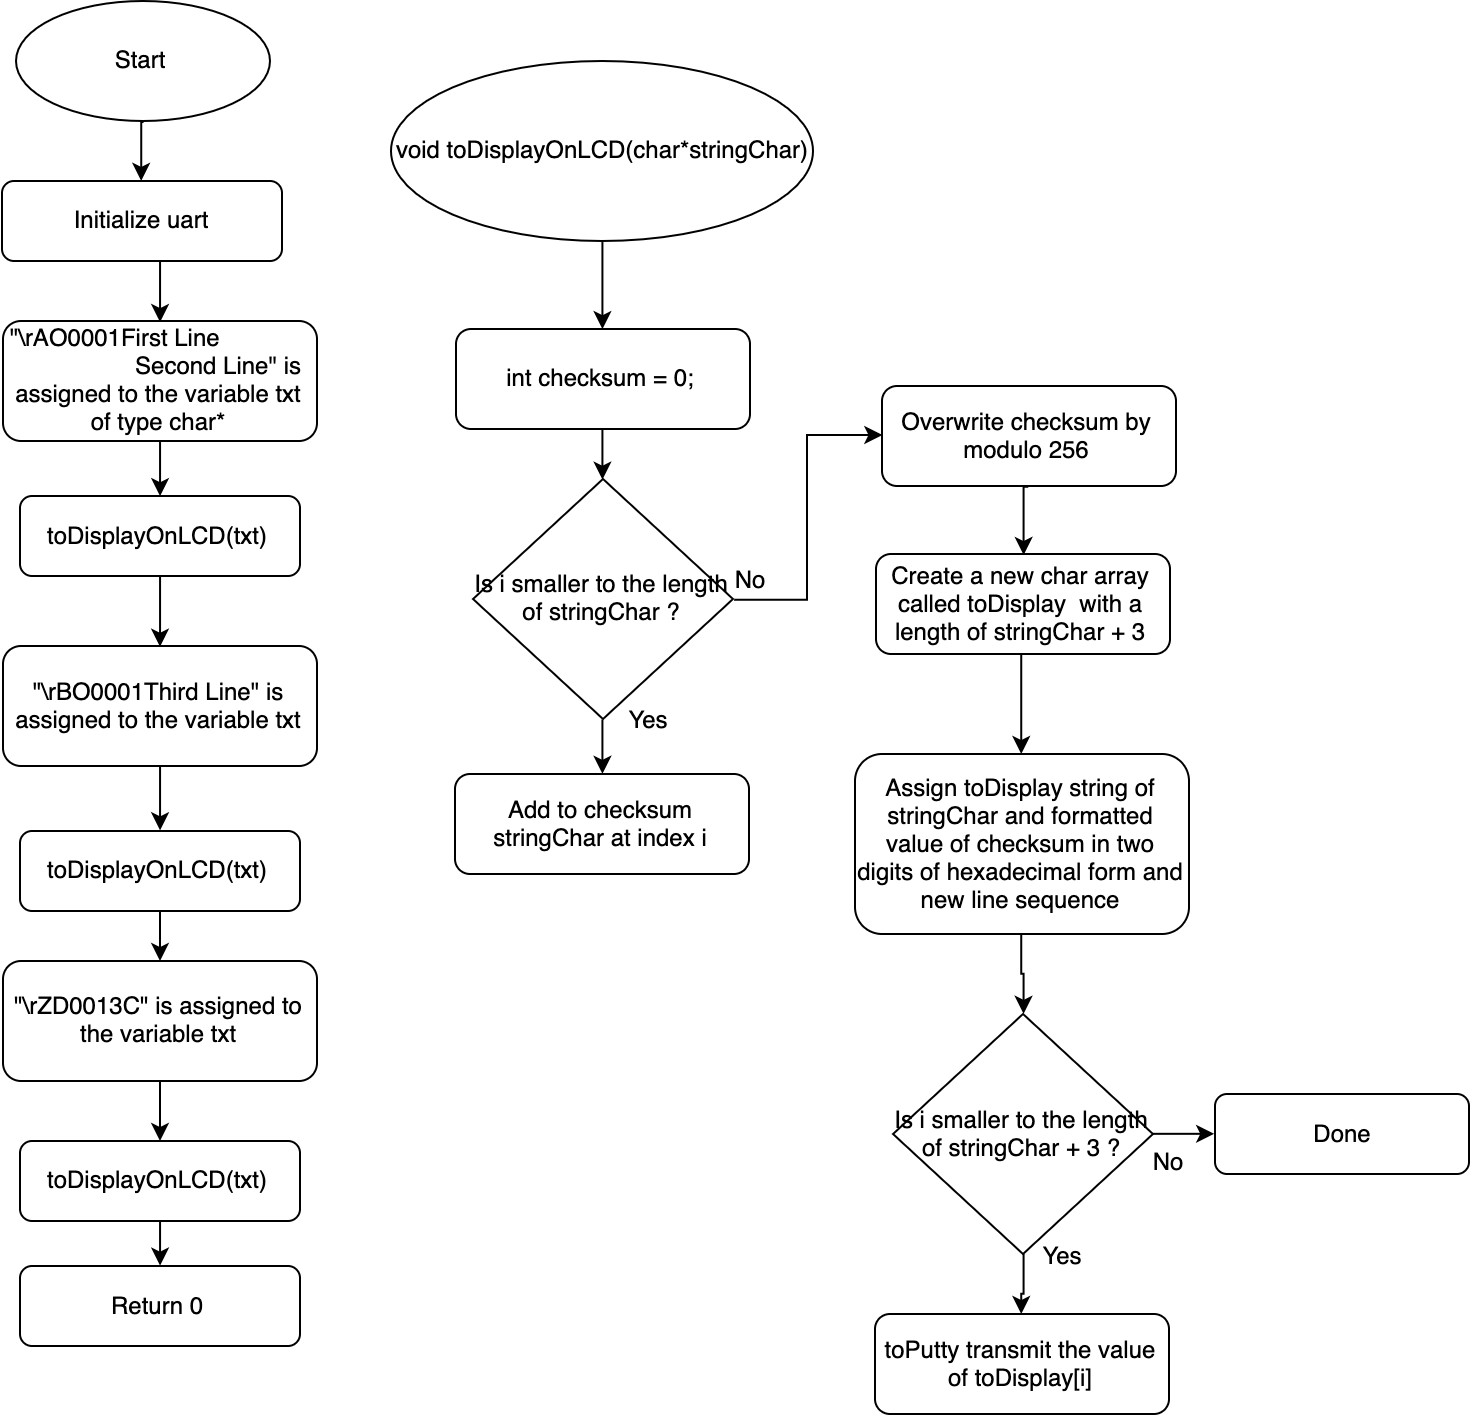
\includegraphics[width=\textwidth/1]{flowchart/task2_flowchart.png}
\end{center}
\caption{Task 2 flowchart}
\label{task2}
\end{figure}

\break

%TASK 3

\section{Task 3}
In this task we used the same methods for void uart\_int(void), void toPutty(unsigned char data) and void toDisplayOnLCD(char* stringChar). 
\lstset{style=CStyle}

\begin{lstlisting}[style=CStyle]
/*>>>>>>>>>>>>>>>>>>>>>>>>>>>>>>>>>>>>>>>>>>>>>>>>>>>>>>>>>>>
; 1DT301, Computer Technology I
; Date: 2016-09-15
; Author:
;    Anas Kwefati
;
; Lab number: 6
; Title: CyberTech Wall Display
;
; Hardware: STK600, CPU ATmega2560
;
; Function: Program that changes text strings on the display.
;
; Input ports: none
;
; Output ports: CyberTech Display.
;
; Subroutines:
; Included files: <avr/io.h> and <util/delay.h>
;
;Other information: Display is connected to the serial port (RS232) on the STK600.
; Communication speed is 2400bps.
;Changes in program: (Description and date)
<<<<<<<<<<<<<<<<<<<<<<<<<<<<<<<<<<<<<<<<<<<<<<<<<<<<<<<<<<<*/
#include <avr/io.h>
#include <stdio.h>
#include <string.h>
#include <stdlib.h>

#define F_CPU 1000000// Clock Speed
#include <util/delay.h>
#define BAUD 2400 //Communication Speed Display rate 2400
#define MYUBBRR (F_CPU/16/BAUD-1) //UBBRR = 25 -> osc = 1MHz and UBRR = 47 -> osc = 1,843200MHz

void uart_int(void);
void toPutty(unsigned char data);
void toDisplayOnLCD(char* stringChar);

int main(void)
{
	uart_int();
	

	char* data = "abc";
	char *txt = "\rAO0001";
	
	for(int i =0;i<strlen(data);i++){
		//The idea is to take char by char and add it one by one to str2
		char c = data[i];
		size_t len = strlen(txt); //take the length of txt
		char *str2 = malloc(len + 1 + 1); //give a length of len and allocate a bit more memory with malloc in case 
		strcpy(str2, txt); // copy txt to str2
		str2[len] = c;  //create an array of str2 with a length of len for the char c
		str2[len + 1] = '\0'; // we add 1 to len and add the end char \0
		toDisplayOnLCD(str2); //call display
		free(str2); //free str2 deallocate the space used by malloc()
		
		str2 = "\rZD0013C";
		toDisplayOnLCD(str2);
		_delay_ms(5000); //wait 5s
	}

		
	return 0; 
}



//METHOD TO DISPLAY ON THE SCREEN 
void toDisplayOnLCD(char* stringChar){
	
	int checksum = 0; 
	 //We make sure that everything is in it
	 for(int i =0; i<strlen(stringChar);i++){
		 checksum += stringChar[i];
	 }
	 
	 checksum\%=256;
	 
	 char toDisplay [strlen(stringChar)+3];
	 sprintf(toDisplay, "\%s\%02X\n", stringChar, checksum); //\%02x means print at least 2 digits, prepends it with 0's if there's less.
	 //\%02x is used to convert one character to a hexadecimal string
	
	for (int i = 0; i<strlen(stringChar)+3;i++){
		toPutty(toDisplay[i]);
	}
}

//INITIALIZATION OF THE DISPLAY 

void toPutty(unsigned char data){
	//WAIT FOR DATA TO BE RECEIVED
	while(!(UCSR1A & (1<<UDRE1)));
	UDR1 = data;
}

void uart_int(void) { 
	UBRR1L = MYUBBRR; //25 because we are setting the board at 1MHz
	/*Enable receiver and transmitter*/
	UCSR1B = (1<<RXEN1|1<<TXEN1); // Receive Enable (RXEN) bit // Transmit Enable (TXEN) bit
}




\end{lstlisting}
\break
\begin{figure}
\begin{center}
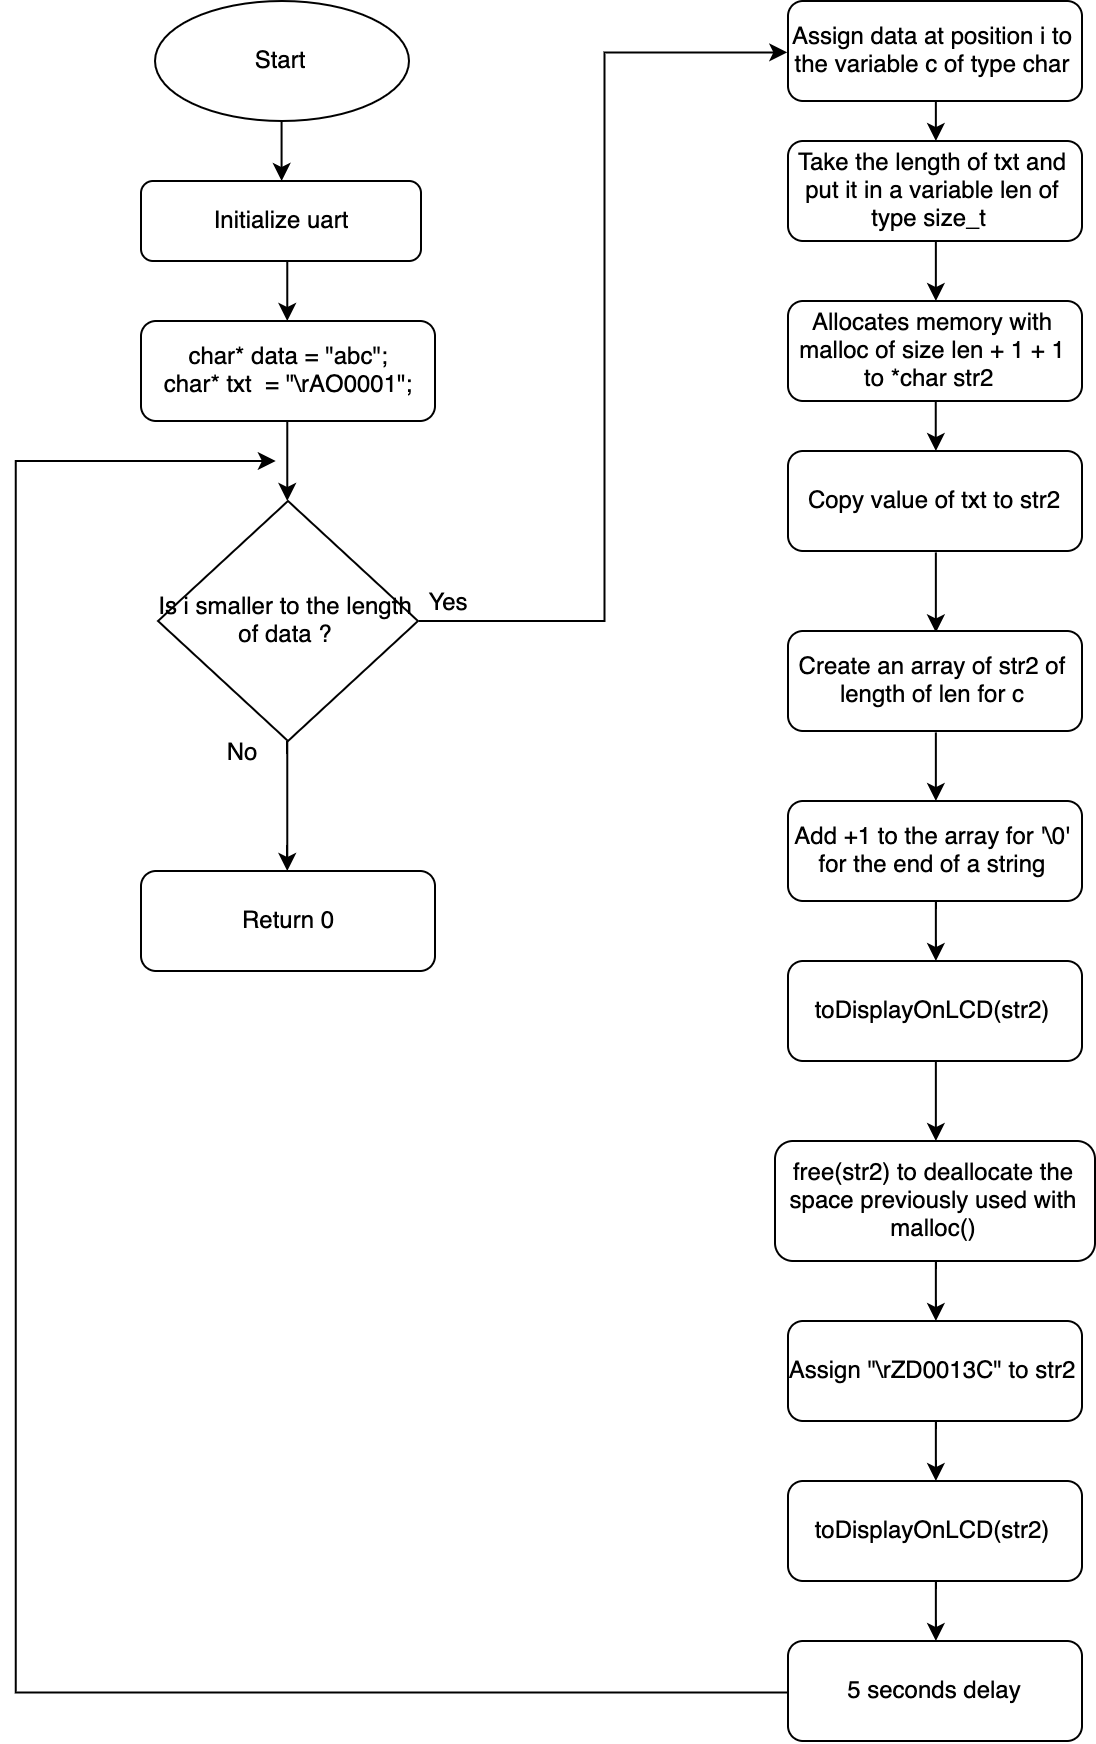
\includegraphics[width=\textwidth/2]{flowchart/task3_flowchart.png}
\end{center}
\caption{Task 3 flowchart}
\label{task3}
\end{figure}

\break

%TASK4
\section{Task 4}

\lstset{style=CStyle}

\begin{lstlisting}[style=CStyle]
/*>>>>>>>>>>>>>>>>>>>>>>>>>>>>>>>>>>>>>>>>>>>>>>>>>>>>>>>>>>>
; 1DT301, Computer Technology I
; Date: 2016-09-15
; Author:
;    Anas Kwefati
;
; Lab number: 6
; Title: CyberTech Wall Display
;
; Hardware: STK600, CPU ATmega2560
;
; Function: Program that communicates with the terminal and the display.
; It is also possible to enter the address on the screen to display text.
;
; Input ports: Serial Port that is connected to the terminal (PuTTY) takes input from keyboard.
;
; Output ports: CyberTech Display.
;
; Subroutines:
; Included files: <avr/io.h> and <util/delay.h>
;
;Other information: Display is connected to the serial port (RS232) on the STK600.
; Communication speed is 2400bps.
; TASK 5 is the same as TASK 4 but with more address to choose (1-9)
;Changes in program: (Description and date)
<<<<<<<<<<<<<<<<<<<<<<<<<<<<<<<<<<<<<<<<<<<<<<<<<<<<<<<<<<<*/
#include <avr/io.h>
#include <stdio.h>
#include <stdlib.h>
#include <string.h>
#include <stdbool.h>

#define F_CPU 1000000// Clock Speed
#include <util/delay.h>
#define BAUD 2400 //Communication Speed Display rate 2400
#define MYUBBRR (F_CPU/16/BAUD-1) //UBBRR = 25 -> osc = 1MHz and UBRR = 47 -> osc = 1,843200MHz
#define MAX_LINES 3 // Possible lines TASK4
#define POSSIBLE_DIGIT_TO_CHOOSE_LINE "123" //TASK4

//#define POSSIBLE_DIGIT_TO_CHOOSE_LINE "123456789" //TASK 5
//#define MAX_LINES 9 //TASK 5 and uncomment the 2 other for TASK 4

void uart_int(void);
void toPutty(unsigned char data);
char getChar();

void improvedtoDisplayOnLCD(char address, char* specialCommand, char* stringChar);
void endToDisplayOnLCD();
void setUpToDisplayOnLCD();

void changeLine (int targetLine);
char possibleCharacter(char* possibleLine, char c);

//SOME GLOBAL VARIABLES
int currentLine = 0;
bool selectionOfLine = false;
char lines[8][24] = { "", "", "", "", "", "", "", "" };//8ROWS 24COLUMNS


int main(void)
{
	uart_int();
	setUpToDisplayOnLCD();
	
	while (1) {
		char character = getChar(); // We get the input from terminal

        //IF SELECT A LINE WE WAIT FOR A VALID DIGIT that is >= 1
		if (selectionOfLine == true) {
            if (character < '1') {
                continue; // If character <1 do nothing
            }
			// We check if the digit that the user has put is in what is possible
			if (possibleCharacter(POSSIBLE_DIGIT_TO_CHOOSE_LINE, character)) {
                int convertCharToInt = character - '0'; //convert char to int
                /*LOGIC behind the conversion :
                 char c = '2';
                 int i = c - '0';
                 it will take the ASCII value of charactter 2 (50) and 0 (48)
                 Then it will substract them -> int i = 50 - 48 which gives us 2
                 */
				changeLine(convertCharToInt); //call the method to choose the possible line. Change currentLine by the targetLine (here "convertCharToInt")
				
                selectionOfLine = false; //False
			}
		}
		else {
			
            if (character == '>'){
                
                selectionOfLine = true; //Make selectionOfLine true
                
            } else if (character == 13 ){
                //Else if character == 'enter'
                changeLine(-1); // We increment currentLine and we go to the next line
                
            } else {
				// Else add character to end of selected line
				char* line = lines[currentLine];
				sprintf(line, "\%s\%c", line, character);
			}
		}
		setUpToDisplayOnLCD(); // Update the screen
	}

	return 0;
}


//INITALIZATION OF THE DISPLAY

void toPutty(unsigned char data){
	//WAIT FOR DATA TO BE RECEIVED and SHOW IT
	while(!(UCSR1A & (1<<UDRE1)));
	UDR1 = data; 
}

void uart_int(void) {
	UBRR1L = MYUBBRR; //25 because we are setting the board at 1MHz
	/*Enable receiver and transmitter*/
	UCSR1B = (1<<RXEN1|1<<TXEN1); // Receive Enable (RXEN) bit // Transmit Enable (TXEN) bit
}

char getChar(){
	//WAIT FOR THE CHARACTER TO BE RECEIVED THEN RETURN IT
	while(!(UCSR1A & (1<<RXC1)));
	return UDR1;
}


//METHOD TO DISPLAY ON THE SCREEN
void improvedtoDisplayOnLCD(char addressLine, char* specialCommand, char* stringChar){
    
	//we get the length of special command which is "O0001"
    //and we get the length of the specific message in stringChar
	int specialCommandLen = sizeof(specialCommand);
	int stringCharLen = sizeof(stringChar);
    
	char* toDisplay = malloc(1 + specialCommandLen + stringCharLen + 3);//give a length of specialCommand and stringCharLen and allocate a bit more memory with malloc for the end case. We allocate memory for toDisplay

	// ADD EVERYTHING TOGETHER in toDiplsay
    //So we get \rADDRESSLINE_SPECIALCOMMAND_STRINGCHAR
    //For example \rAO0001a"
	sprintf(toDisplay, "\r\%c\%s\%s", addressLine, specialCommand, stringChar);

	
    int checksum = 0;
    // We calculate checksum to make sure that everything is in it
	for (int i = 0; (toDisplay[i] != 0); i++){
		checksum += toDisplay[i];
	}
	
	checksum \%= 256;

	sprintf(toDisplay, "\%s\%02X\n", toDisplay, checksum);//\%02x means print at least 2 digits, prepends it with 0's if there's less.
    //\%02x is used to convert one character to a hexadecimal string

	for (int i = 0; (toDisplay[i] != 0); i++){
		toPutty(toDisplay[i]);
	}
	

	free(toDisplay); // free toDisplay deallocate the space used by malloc()
}

void endToDisplayOnLCD(){
    char* txt = "\rZD0013C\n";
    for(int i = 0; i<strlen(txt);i++){
        toPutty(txt[i]);
    }
}



//METHOD TO SETUP CHARACTERS FOR EACH LINE
void setUpToDisplayOnLCD(){
    
	//Take currentLine and see if it is <1 if yes then increment lineToDisplay
	int lineToDisplay = currentLine;
    
    if (lineToDisplay < 1){
        lineToDisplay++;
    }
	
	
	//Set up for first and second rows
	char memory_space_A[48] = "";
    
	//char line_selected = selectionOfLine ? '_' : (currentLine + '0');
    
    //If ChooseALine is True then add '_' to choosenLine otherwise the currentLine

    char choosenLine = "";
    if(selectionOfLine == true){
        choosenLine = '_';
    } else {
        choosenLine = currentLine + '0';
    }

    //Add everything in the array of char.
	sprintf(memory_space_A, "Choose input: \%c         \%s", choosenLine, lines[lineToDisplay-1]);

	// Set up for third row
	char memory_space_B[48] = " ";
    if (lines[lineToDisplay][0] == true){
        continue; //check if the selected like is '\0', if yes then do nothing
       
    }
    
    for (int i = 0; i < 48; i++){
        //Send data from third row to the memory
        //memory_space_B[i] = lines[1][i]
        memory_space_B[i] = lines[lineToDisplay][i];
    }
	
	// Send everything to improvedtoDisplayOnLCD to do the calculation with checksum then it will send it to the screen
	improvedtoDisplayOnLCD('A', "O0001", memory_space_A);
	improvedtoDisplayOnLCD('B', "O0001", memory_space_B);
    endToDisplayOnLCD();
}




//METHOD TO CHECK IF THE USER INPUT IS ALLOWED TO CHOOSE LINE
char possibleCharacter(char* possibleLine, char c){
    char tempChar;
    
    //While will continue until the character is \0
    while (*possibleLine){
        tempChar = *possibleLine; //We take char by char from possibleLine and we add it to the char t
        
        if (tempChar == c) {
            //In this condidition, we check if tempChar is equal to the user input c
            return 1; //return 1 if yes
        }
        possibleLine++; //increment possibleLine to go to the next possible char defined by us at the beginning
    }

    return 0; //0 if not
}



// METHOD TO CHOOSE LINE BY INCREMENTS OR NOT
void changeLine (int targetLine){
    
    //if targetLine == -1 then we increase currentLine by 1
    //By default currentLine == 0
    //So if we press 'enter' it will increase currentLine by 1
    //Hence currentLine == 1. And it does this as long as we don't reach the maximum of line possible
	if (targetLine == -1) {
		currentLine++;
        if (currentLine >= MAX_LINES){
            currentLine = 0; //We reset the currentLine to 0 when it exceeds the maximum possible lines.
        }
		
	}
    else {
        // change to selection
        currentLine = targetLine;
    }
}



\end{lstlisting}


\begin{figure}
\begin{center}
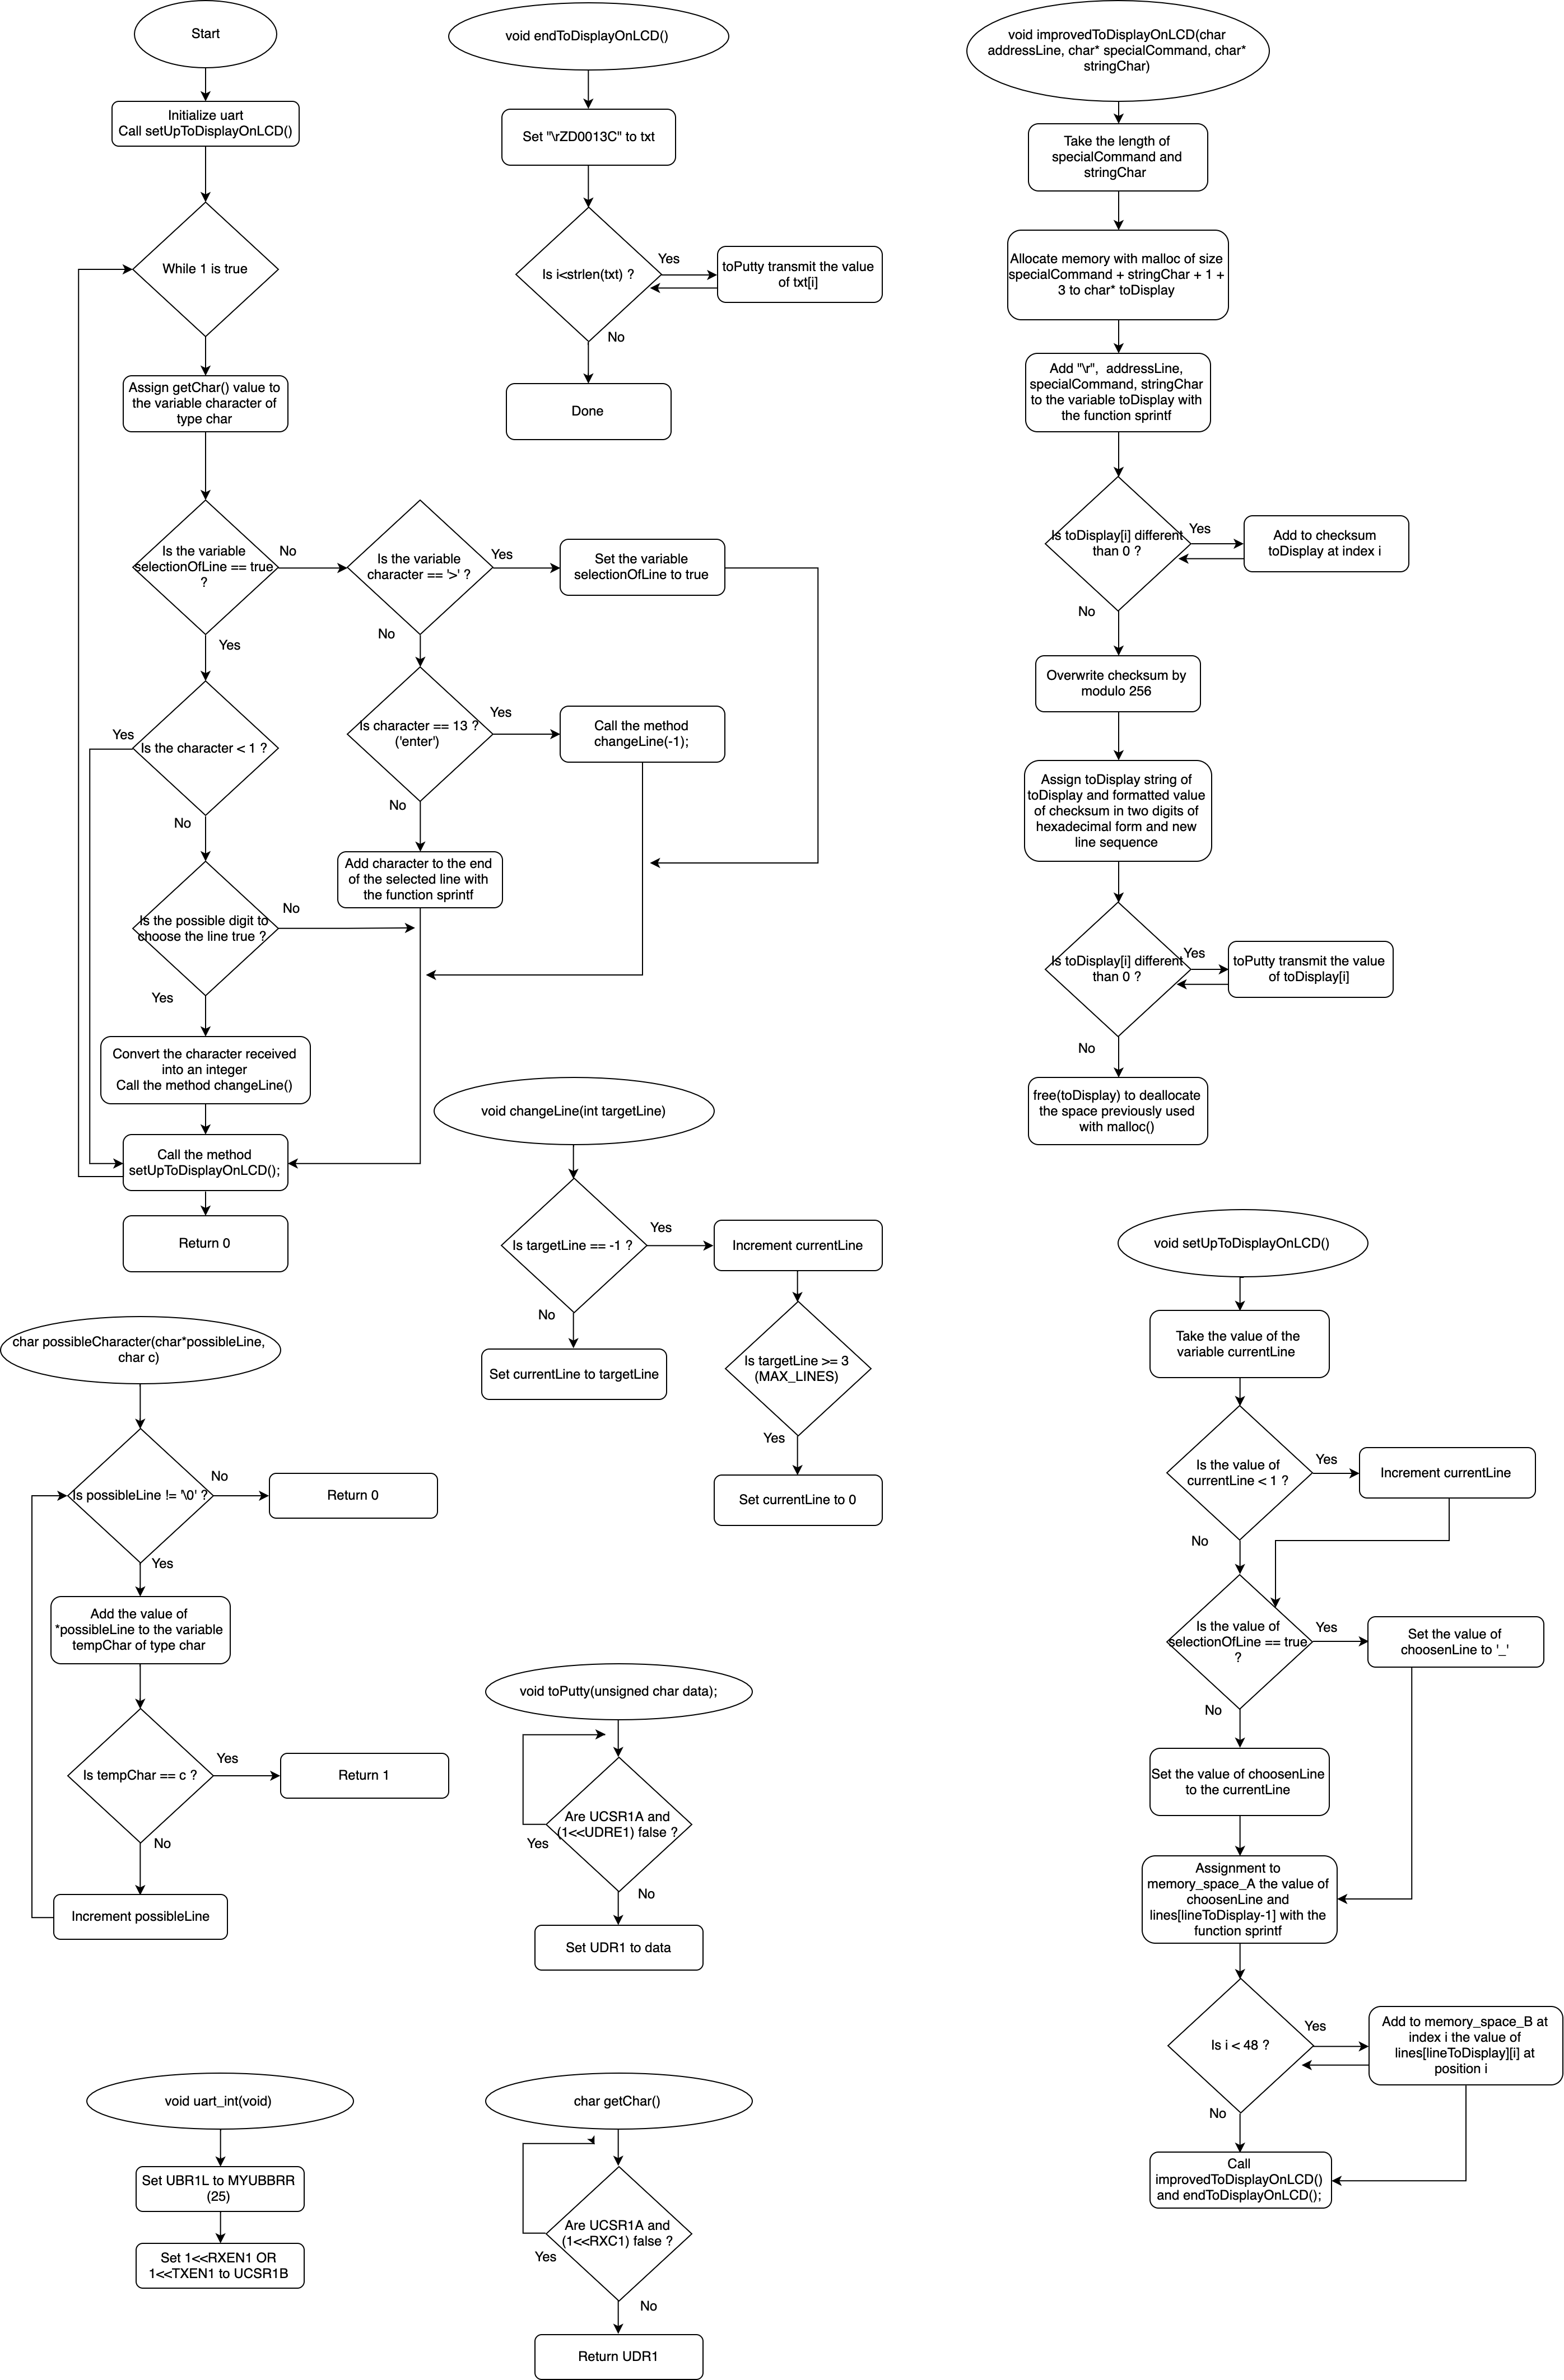
\includegraphics[width=\textwidth/1 ]{flowchart/task4_flowchart.png}
\end{center}
\caption{Task 4 flowchart}
\label{task4}
\end{figure}

\break
%TASK5
\section{Task 5}
Task 5 is the same as Task 4 but with more addresses to choose. (1 to 9). Therefore the flowchart of task 5 is the same as task 4.
\lstset{style=CStyle}

\begin{lstlisting}[style=CStyle]

\end{lstlisting}






% Prints your bibliography database xxx.bib
\bibliographystyle{IEEEtran}
\bibliography{ref.bib}

\end{document}
